% Template:     Presentación LaTeX
% Documento:    Archivo principal
% Versión:      1.4.5 (27/09/2021)
% Codificación: UTF-8
%
% Autor: Pablo Pizarro R.
%        pablo@ppizarror.com
%
% Manual template: [https://latex.ppizarror.com/presentacion]
% Licencia MIT:    [https://opensource.org/licenses/MIT]

% CREACIÓN DEL DOCUMENTO
\pdfminorversion=7
\documentclass[
	spanish, % Idioma: spanish, english, etc.
	aspectratio=43, % 1610, 169, 149, 54, 43, 32
	hyperref={pdfencoding=auto,psdextra},
	xcolor={dvipsnames,table,usenames},
]{beamer}

% INFORMACIÓN DEL DOCUMENTO
\def\documenttitle {Modelamiento y seguimiento de tópicos para detección de modus operandi en robo de vehículos}
\def\documentsubtitle {Modelamiento dinámico de tópicos}
\def\documentsubject {Tesis para optar al grado de Magíster en Gestión de Operaciones \newline Memoria para optar al título de Ingenierio Civil Industrial}

\def\documentauthor {Diego Garrido}
\def\coursename {}
\def\coursecode {}

\def\universityname {Universidad de Chile}
\def\universityfaculty {Facultad de Ciencias Físicas y Matemáticas}
\def\universitydepartment {Departamento de Ingeniería Industrial}
\def\universitydepartmentimage {departamentos/fcfm}
\def\universitylocation {Santiago de Chile}

% CONFIGURACIÓN DATOS BEAMER
\title[\documentsubtitle]{\documenttitle}
\subtitle{\documentsubject}
\author[\documentauthor]{
	\documentauthor \newline\newline
Profesor guía: Richard Weber \newline
Miembros de la comisión: Ángel Jiménez, Giorgiogiulio Parra
}
\institute[UChile]{
	\includegraphics[height=1.1cm]{\universitydepartmentimage} \\
	\medskip
	\universityname \\
	\universityfaculty \\
	\universitydepartment
}
\date[\today]{\footnotesize{\today}}

% IMPORTACIÓN DEL TEMPLATE
\input{template}

% INICIO DE LAS PÁGINAS
\begin{document}

% CONFIGURACIÓN DE PÁGINA Y ENCABEZADOS
\templatePagecfg

% CONFIGURACIONES FINALES
\templateFinalcfg

\newcommand\blfootnote[1]{%
  \begingroup
  \renewcommand\thefootnote{}\footnote{#1}%
  \addtocounter{footnote}{-1}%
  \endgroup
}

\definecolor{royalblue}{HTML}{214ED3}
% ======================= INICIO DEL DOCUMENTO =======================
\begin{frame}
	\titlepage
\end{frame}


\begin{frame}
	\frametitle{Contenidos}
	\tableofcontents
\end{frame}


\section{Motivación}

\begin{frame}[t]
\frametitle{Motivación: Metodología}
  
\begin{columns}
\column{0.5\textwidth}
\begin{itemize}
  \item Incremento de volumenes de datos requiere métodos automáticos de análisis\footnote{\url{https://www.sigmacomputing.com/blog/top-20-big-data-statistics/}}.
     \begin{enumerate}
      \item Al día \textbf{2 EB} de datos son generados.
      \item Un \textbf{80\%} es no estructurado.
      \item Tan solo un \textbf{12\%} es analizado.
    \end{enumerate}
  \item 
    El modelamiento de tópicos permite resumir y organizar grandes colecciones de texto. %Ejemplo: descubrimiento de nuevos tipos de accidentes de trayecto apartir de relatos de accidentes laborales. Como accidentes de trayecto causado por mascarillas.
    \item Este trabajo es una propuesta de modelamiento de tópicos dinámico: nacimiento, muerte, evolución, división y fusión de tópicos.
  \end{itemize}

\column{0.5\textwidth}
\begin{figure}
  \includegraphics[width=1.0\textwidth]{covid_research.jpg} 
 \end{figure}
 \end{columns}
\end{frame}

\begin{frame}[t]
\frametitle{Motivación: Caso de estudio} 

El problema del robo de vehículos o accesorios de vehículos afecta a toda la sociedad en Chile y en el mundo. 
\begin{columns}

\column{0.5\textwidth}
Algunos de sus efectos son:
  \begin{itemize}
    \item Incremento en la percepción de seguridad.
    \item Aumento en la prima de los seguros de los asegurados.
    \item Aumento en los costos de las aseguradoras.
    \item Incremento en otro tipos de delitos.
    \item problema que se ha vuelto más relevante el último tiempo debido al crecimiento en el robo de vehículo motorizado y accesorios. 
  \end{itemize}
 
\column{0.5\textwidth}
\begin{figure}
    \includegraphics[width=1.0\textwidth]{robberies.eps} 
    \caption{Cantidad de robos de vehículos y accesorios anuales en Chile entre los años 2006-2016. Fuente: Informe anual de Carabineros, 2006-2016, INE.} 
    \label{fig:antecedente}
\end{figure}

\end{columns}
\end{frame}




\section{Revisión del estado del arte}

\begin{frame}[t]
\frametitle{Revisión del estado del arte: ¿Qué es el modelamiento de tópicos?}
  El modelamiento de tópicos es uno de los enfoques más prometores de \textit{clustering} aplicado a texto, siendo su objetivo descubrir los temas (\textit{clusters}) ocultos presentes en el corpus, permitiendo \textbf{resumir}, \textbf{organizar} y \textbf{explorar} grandes colecciones de datos.

\begin{figure}
\insertimage{topic_modelling.png}{scale=0.3}{Intuición detrás de Latent Dirichlet Allocation. Fuente: Figura 1 de \cite{blei2012probabilistic}.}
\end{figure}

\end{frame}


\begin{frame}[t]
\frametitle{Revisión del estado del arte: Tipos de modelos de tópicos}
Las técnicas de modelamiento de tópicos suelen estar basadas en \textbf{factorización matricial} o en \textbf{modelos probabilísticos generativos}. 
\newline\newline
A continuación algunos ejemplos de ambos enfoques:

\begin{itemize}
  \item \textbf{LSI} (Latent Semantic Indexing) \cite{dumais2004latent} o \textbf{NMF} (Non-negative Matrix Factorization)\cite{xu2003document}. 
  \item \textbf{LDA} (Latent Dirichlet Allocation)\cite{blei2003latent} o \textbf{HDP} (Hierarchical Dirichlet Process)\cite{teh2005sharing}. 
\end{itemize} 

Este trabajo aborda el enfoque probabilístico: 
\begin{itemize}
  \item \textbf{Expresa incertidumbre} en la asignación de un tópico a un documento y en la asignación de palabras a los tópicos.
  \item Suele aprender \textbf{tópicos más descriptivos} \cite{stevens2012exploring}.
\end{itemize}

\end{frame}


\begin{frame}[t]
\frametitle{Revisión del estado del arte: Modelamiento dinámico}
En el modelamiento de tópicos se pueden presentar los siguientes dinámismos:

\begin{enumerate}
  \item \textbf{Evolución de tópicos.}
  \item \textbf{Dinámismo en la mezcla de tópicos.}
  \item \textbf{Nacimiento, muerte, fusión y división de tópicos.}
\end{enumerate}

Dentro de los modelos de tópicos dinámicos se tiene:
\begin{itemize}
  \item \textbf{DTM} (Dynamic Topic Modelling)\cite{blei2006dynamic} y \textbf{TOC} (Topic Over Time)\cite{wang2006topics} \textbf{permiten el punto 1 y 2} manteniendo fijo el número de topicos en el tiempo.
  \item \textbf{DHDP} (Dynamic Hierarchical Dirichlet Process)\cite{ahmed2012timeline} \textbf{captura el punto 1, 2 y 3 parcialmente}, con excepción de fusión y división. \textbf{No cuenta con una implementación}.\\
  \item En \cite{wilson2011tracking} y \cite{beykikhoshk2018discovering} se capturan los dinámismos mencionados dividiendo el corpus en épocas, entrenando de forma independiente un modelo por época para finalmente unificar (LDA y HDP).
\end{itemize}
\end{frame}


\section{Metodología propuesta}

\begin{frame}[t]
\frametitle{Metodología propuesta}
\begin{enumerate}
  \item División del corpus en épocas siendo cada época preprocesada de forma independiente. 
  \item Aplicación de HDP en cada época de manera independiente. 
  \item Construcción del grafo de similitud WMD entre épocas adyacentes y eliminación de arcos con similitud menor al cuantil $\zeta$ de la \textbf{cdf}.
\end{enumerate}

\vspace*{-0.1in}
\begin{figure}
\insertimage{methodology.png}{scale=0.18}{}
\caption{Esquema de la metodología de descubrimiento y evolución de tópicos.}
\label{img:scheme}
\end{figure}

\end{frame}


\begin{frame}[t]
\frametitle{Metodología propuesta: Hierarchical Dirichlet Process}
\textbf{HDP} (Hierarchical Dirichlet Process) es un \textit{prior} jerárquico no paramétrico formado por un DP cuya medida base $G_{0}$ es dibujada a partir de otro DP.

\vspace*{-0.1in}
\begin{figure}
\begin{columns}
  \begin{column}{0.5\textwith}
  \hspace*{-3cm}\vbox{\begin{aligned}
         H \quad &= \quad \text{Dir}(\frac{\eta}{|V|}1_{|V|})\\
         G_{0}|\gamma, H \quad &\sim \quad \text{DP}(\gamma, H)\\
         G_{d}|\alpha, G_{0} \quad &\sim \quad \text{DP}(\alpha_{0}, G_{0})\\
         \phi_{d,n}|G_{d} \quad &\sim \quad G_{d}\\
         w_{d,n}|\phi_{d,n} \quad &\sim \quad \text{Cat}(\phi_{d,n})
  \end{aligned}}
  \end{column}
  \begin{column}{0.5\textwith}
  \hspace*{-10em}\raisebox{2em}{\scalebox{0.8}{
      \tikz{ %
      \node[latent, dashed] (H) {$H$} ; %
      \node[latent, right=of H] (G0) {$G_{0}$} ; %
      \node[latent, above= of G0, dashed] (gamma) {$\gamma$} ; %
      \node[latent, right=of G0] (Gd) {$G_{d}$} ; %
      \node[latent, above= of Gd, dashed] (alpha0) {$\alpha_{0}$} ; %
      \node[latent, right= of Gd] (phi) {$\phi_{d,n}$} ; %
      \node[obs, right=of phi] (w) {$w_{d,n}$}   ; %
      \plate[inner sep=0.25cm, xshift=-0.12cm, yshift=0.12cm] {plate1} {(phi) (w)} {$N_{d}$}; %
      \plate[inner sep=0.25cm, xshift=-0.12cm, yshift=0.12cm] {plate2} {(Gd) (plate1)} {$D$}; %
      \edge {H, gamma} {G0} ; %
      \edge {G0, alpha0} {Gd} ; %
      \edge {Gd} {phi} ; %
      \edge {phi} {w} ; %
      }
    }}
\caption{Representación gráfica de HDP: círculos denotan variables aleatorias, círculos abiertos denotan parámetros, círculos sombreados denotan variables observadas y los platos indican replicación.}
\end{column}
\end{columns}
\end{figure}

La discretitud de $G_{0}$ asegura:
  \begin{itemize}
    \item \textbf{A nivel del corpus} los documentos comparten el mismo \textbf{conjunto de tópicos} (\textit{mixture components}). 
    \item \textbf{A nivel del documento} $G_{d}$ hereda los tópicos de $G_{0}$, pero los \textbf{pesos de cada tópico} (\textit{mixture proportions}) es específica del documento.
  \end{itemize}
\end{frame}


\begin{frame}[t]
\frametitle{Metodología propuesta: Construcción del grafo de similitud temporal}
\begin{itemize}
  \item Construcción del grafo \textit{fully connected} de las similitudes entre tópicos de épocas adyacentes ($\phi_{t,i}$ y $\phi_{t+1,j}$) usando una medida de similitud $\rho \in [0,1]$.
  \item Eliminación de las conexiones débiles en base a un umbral $\alpha \in [0,1]$, reteniendo solo aquellas conexiones que cumplen $\rho(\phi_{t,i}, \phi_{t+1,j})\leq \alpha$.
\end{itemize}

\vspace*{-0.3in}
\begin{figure}
\insertimage{similarity_graph.png}{scale=0.12}{}
\caption{Ilustración conceptual del grafo de similitud que modela la dinámica de los tópicos en el tiempo. Un nodo corresponde a un tópico en una época específica; el ancho de los arcos es proporcional a la similitud entre los tópicos, arcos ausentes fueron eliminados por presentar una similitud menor a un umbral. Fuente:  Figura 3 de \cite{beykikhoshk2018discovering}.}
\label{img:graph}
\end{figure}		

\end{frame}


\begin{frame}[t]
\frametitle{Metodología propuesta: Prunning}

\begin{itemize}
  \item El umbral de corte es el cuantil $\zeta \in [0,1]$ de la cdf de las similitudes ($F_{p}$), es decir, $F_{p}^{-1}(\zeta)$.
  \item El úmbral de corte no es arbitrario según la médida de similitud escógida.
\end{itemize}

\vspace*{-0.3in}
\begin{figure}
  \insertimage{cdf_sim.png}{scale=0.15}{}
  \caption{Estimación empírica de la función de densidad acumulada (cdf) de la similitud entre tópicos de épocas adyacentes en un grafo \textit{fully-connected} para tres medidas de similitud. Fuente: Figura 4 \cite{beykikhoshk2018discovering}.}
  \label{img:cdf_sim}
\end{figure}

\end{frame}


\begin{frame}[t]
\frametitle{Metodología propuesta: Word Mover's Distance}

\begin{itemize}
  \item \textbf{WMD} (Word Mover's Distance) \cite{kusner2015word}: distancia que permite comparar vectores sin vocabulario común ya que trabaja sobre el espacio de los \textit{word embeddings}. 
  \item Sea  $V_{i}$ y $V_{j}$ los vocabularios del tópico $i$ y $j$ respectivamente, luego se tiene $WMD(\phi_{i}, \phi_{j})$:
\end{itemize}

\vspace*{-0.4in}
\begin{columns}
\begin{column}{0.4\textwidth}

\begin{align}
\underset{x}{\text{min}}&\sum_{u \in V_{i}}\sum_{v \in V_{j}} c_{u,v}x_{u,v} \\ 
\textrm{s.t.} &\sum_{v \in V_{j}}x_{u,v}= \phi_{i,u}, \; u \in V_{i}\\ 
& \sum_{u \in V_{i}}x_{u,v}= \phi_{j,v}, \; v\in V_{j}\\
& x_{u,v} \geq 0,\; u \in V_{i} \;, v \in V_{j}\\ \nonumber
\end{align}

\end{column}

\begin{column}{0.6\textwidth}
\begin{figure}
\insertimage{wmd-obama.png}{scale=0.15}{}
\caption{Espacio vectorial de los \textit{word embeddings} de las palabras de dos documentos con un vocabulario de tamaño 4. Fuente: Figura de \cite{WMDPy}.}
\label{img:wmd_obama}
\end{figure}
\end{column}

\end{columns}
  WMD se puede transformar en médida de similitud\footnote{Notar que WMD es 0 si la similitud es 1 e $\infty$ si la similitud es 0.} considerando $\rho(\phi_{i}, \phi_{j}) = \frac{1}{1+WMD(\phi_{i}, \phi_{j})}$.

\end{frame}


\begin{frame}[t]
\frametitle{Metodología propuesta: WMD complejidad}

WMD es una medida de distancia \textbf{intensiva en recursos computacionales}.\newline

Usando el algoritmo desarrollado por \cite{pele2009fast} se tiene que el mejor tiempo promedio escala $\mathcal{O}(N^{2}log N)$, donde $N$ es el tamaño del vocabulario entre dos épocas adyacentes.
  \begin{align*}
\{x| Ax=b, x\geq 0\}, A\in \mathbb{R}^{2N\times N^{2}}, b\in \mathbb{R}^{2N}, x\in \mathbb{R}^{N}
  \end{align*}

Se requiere de \textbf{heurísticas} para acelerar el tiempo de computo.
\begin{itemize}
  \item Los tópicos siguen una distribución con forma de \textbf{ley de potencia} sobre el vocabulario, donde una pequeña fracción de las palabras concentran la mayor parte de la masa de la distribución. 
  \item En la práctica \textbf{la interpretación de los tópicos se basa en los top $N$ palabras más probables}, usualmente con $N \in [5, 30]$, entonces, se puede aprovechar esta estructura para efectos de computar la WMD de un forma más eficiente, por ejemplo, utilizando solo las palabras que capturan un determinado porcentaje de la distribución acumulada del tópico.
\end{itemize}
\end{frame}


\begin{frame}[t]
\frametitle{Metodología propuesta: Configuración de hiperparámetros}

HDP cuenta con tres hiperparámertos:
\begin{itemize} 
  \item El \textbf{parámetro de concentración a nivel corpus $\gamma$} y el \textbf{parámetro de concentración a nivel documento $\alpha_{0}$}. En \cite{teh2005sharing} los parámetros de concentración se integran afuera usando un prior \textit{vague gamma} \cite{escobar1995bayesian}. En este caso se utilizó un prior $\Gamma(\alpha=1, \beta=1)$.
  \item El \textbf{parámetro de la medida base Dirichlet $\eta$}. Se prefiere usar $\eta\in (0,1)$ ya que genera distribuciones \textit{sparse} sobre el vocabulario. En este caso se utilizó un punto intermedio, fijando $\eta=0.5$.
\end{itemize}

El grafo temporal cuenta con dos hiperparámetros:
\begin{itemize}
  \item \textbf{$q \in [0,1]$ cuantil de corte de la cdf del tópico}. Se prefieren valores en $[0.8, 0.95]$ ya que conservan el \textit{core} de palabras del tópico y disminuye significativamente el tiempo de cómputo.
  \item \textbf{$\zeta\in[0,1]$ cuantil de corte de la cdf de las similitudes del grafo \texix{fully connected}}. Se prefieren valores en $[0.9, 0.99]$ ya que se conservan aquellas relaciones con alta similitud relativa.
\end{itemize}

\end{frame}


\section{Caso de estudio}

\begin{frame}[t]
\frametitle{Caso de estudio: Corpus}

El corpus provisto por la Asociación de Aseguradores de Chile (AACH) consta de 49,015 relatos de víctimas del robo de vehículos provistos entre los años 2011-2016.


\def\grayboxtext[#1,#2]#3{
        \node[fill=gray!80, text width=18em, draw=black!80, rounded corners, align=justify, below=#1] (#2) {#3}; 
}

\begin{columns}[t]
\begin{column}{0.5\textwidth}
\begin{figure}
\begin{tikzpicture}
    \grayboxtext[0.2cm of t3,t4]{\small Descripción Siniestro: el dia 24 de abril se le arrendo el vh a XX el cual estuvo sin problemas pagando el arriendo  hasta el mes pasado que no pago mas y se le ha llamado en reiteradas veces y dice que va a venir a dejar el auto y no aparecel. por eso se realizo una denuncia por apropiacion indevida};
    \grayboxtext[0.2cm of t4,t5]{\small ammg  53966748    vh asegurado transitaba en calle copiapo alt. 750  en este punto sufro portonazo sujetos armados roban mi vh hoy a las 04.30am vh fue encontrado en sector de la pintana mi vh ahora esta siendo periciado.    daños por evaluar};
\end{tikzpicture}
\caption{Muestra de relatos de la base de datos AACH.}
\label{img:documents}
\end{figure}
\end{column}

\begin{column}{0.5\textwidth}
\begin{figure}
\includegraphics[width=1.0\textwidth]{robberies_aach.eps}
\caption{Cantidad de robos registrados por año en base de datos AACH.} 
\label{fig:antecedente}
\end{figure}
\end{column}
\end{columns}

\end{frame}


\begin{frame}[t]
\frametitle{Caso de estudio: Preprocesamiento}

\begin{columns}[t]
\begin{column}{0.5\textwidth}
\begin{table}[H]
    \begin{tabular}{|c|c|c|c|}
    \hline
    procesamiento & documentos & vocabulario & tokens  \\ \hline
    t             & 49,015      & 93,203       & 2,030,980 \\ \hline
    t+ch          & 49,003      & 42,921       & 1,028,412 \\ \hline
    t+ch+f        & 48,988      & 3,148        & 925,693  \\ \hline
    t+ch+f+v      & 48,988      & 2,902        & 901,745  \\ \hline
    t+ch+f+v+s    & 48,566      & 1,960        & 495,182  \\ \hline
    t+ch+f+v+s+d  & 38,850      & 1,960        & 453,206  \\ \hline
    \end{tabular}
\end{table}

\begin{table}[H]
    \begin{tabular}{|c|r|r|r|r|}
    \hline
    \textbf{época} & \multicolumn{1}{c|}{\textbf{t-1}} & \multicolumn{1}{c|}{\textbf{t}} & \multicolumn{1}{c|}{\textbf{t-1 {[}\%{]}}} & \multicolumn{1}{l|}{\textbf{t {[}\%{]}}} \\ \hline
    2              & 1,145                              & 1,187                            & 14.41                                      & 18.08                                    \\ \hline
    3              & 1,187                              & 1,281                            & 13.56                                      & 21.48                                    \\ \hline
    4              & 1,281                              & 1,329                            & 13.35                                      & 17.10                                    \\ \hline
    5              & 1,329                              & 1,405                            & 12.57                                      & 18.28                                    \\ \hline
    6              & 1,405                              & 1,537                            & 10.25                                      & 19.64                                    \\ \hline
    \end{tabular}
\end{table}
\end{column}

\begin{column}{0.5\textwidth}
\begin{figure}
\includegraphics[trim={1.155cm 1.3cm 0 0},clip,width=0.8\textwidth]{cum_dist_1.eps}
\end{figure}

\begin{figure}
\includegraphics[trim={1.155cm 1.3cm 0 0},clip,width=0.8\textwidth]{cum_dist_6.eps}
\end{figure}
\end{column}
\end{columns}

\end{frame}


\begin{frame}[t]
\frametitle{Caso de estudio: CDF del grafo fully-connected}

\begin{figure}
\includegraphics[width=0.8\textwidth]{cdf.eps}
\caption{Estimación empírica de la cdf de la similitud WMD entre tópicos del grafo \textit{fully-conected}.}
\label{img:cdf_wmd}
\end{figure}

\end{frame}


\begin{frame}[t]
\frametitle{Caso de estudio: Grafo de similitud temporal}

\vspace*{-0.2in}
\begin{figure}
\subfloat[$\zeta$ = 0]{
  \includegraphics[width=0.35\textwidth]{graph_q100.png}
}
\subfloat[$\zeta$ = 0.9]{
  \includegraphics[width=0.35\textwidth]{graph_q100_e90.png}
}\\
\subfloat[$\zeta$ = 0.95]{
  \includegraphics[width=0.35\textwidth]{graph_q100_e95.png}
}
\subfloat[$\zeta$ = 0.99]{
  \includegraphics[width=0.35\textwidth]{graph_q100_e99.png}
}
\caption{Grafos temporales con WMD como medida de similitud bajo diferentes puntos operantes $\zeta$ de la CDF. El eje horizontal denota el tiempo en años, partiendo en el 2011 hasta el 2016, donde cada columna de tópicos corresponde a una época específica. Mientras más claro sea el color del nodo que representa un tópico más popularidad posee en su correspondiente época y mientras mayor es el grosor del arco entre dos tópicos mayor es su similitud.}
\label{img:temporal_similarity_graphs}
\end{figure}

\end{frame}


\begin{frame}[t]
\frametitle{Caso de estudio: Efecto del punto operante en el dinámismo}

\begin{figure}

\vspace*{-0.2in}
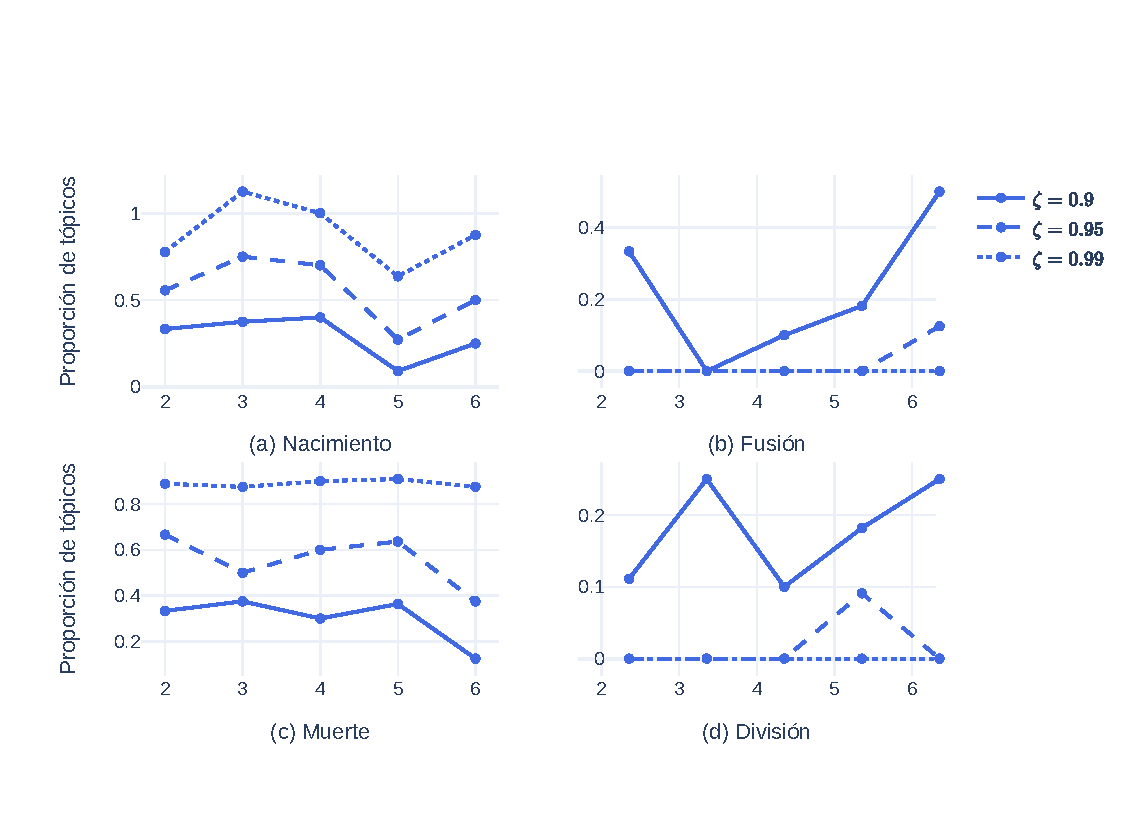
\includegraphics[width=0.8\textwidth]{topics_evolution.eps}
\caption{Proporción de tópicos que nacen, mueren, fusionan y dividen por época, normalizando por el número total de tópicos inferido en esa época, bajo diferentes puntos operantes $\zeta$.}
\label{img:topics_evolution}
\end{figure}

\end{frame}


\begin{frame}[t]
\frametitle{Caso de estudio: Trade off entre precisión y speedup}
 
\vspace*{-0.2in}
\begin{figure}
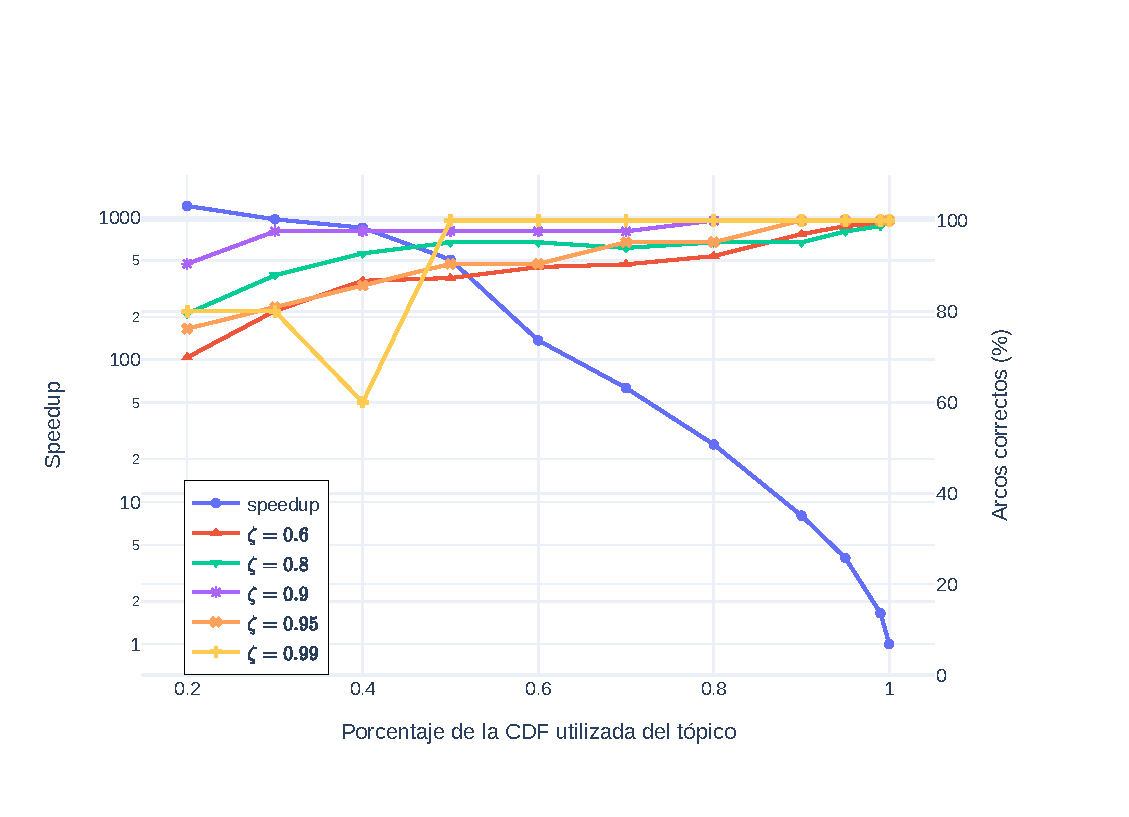
\includegraphics[width=0.8\textwidth]{speedup.eps}
\caption{\textit{Speedup} y porcentaje de arcos correctos al utilizar un menor porcentaje de la cdf de los tópicos en la construcción del grafo de similitud. El error de la heurística es mostrado para diferentes puntos operantes $\zeta$ utilizados para podar el grafo completo.} 
\label{img:speedup}
\end{figure}

\end{frame}


\begin{frame}
\frametitle{Caso de estudio: Evolución del robo no presencial}

El tópico presenta una tendencia a la baja en su participación, en el año 2011 alrededor del 44\% \textit{tokens }provienen de este tópico y en el año 2016 se tiene un 32\%.

\def\topic[#1,#2,#3]#4{
        \node[fill=#1, rounded corners, minimum height=40, minimum width=50, text width=1em] (#2) at #3 {}; 
        \node[anchor=north,inner sep=2pt,] at (#2.north)  {\fontsize{0.18cm}{0.2cm}\selectfont #4};
}
\def\tedge[#1,#2,#3,#4,#5];{ 
  \definecolor{color0}{RGB}{153,153,153}
  \draw[color=color0,#4,fill=white, line width=4*#5pt] (#1) -- #3
  (#2);  
}

\definecolor{color1}{RGB}{184,222,41}
\definecolor{color2}{RGB}{253,231,37}
\definecolor{color3}{RGB}{134,213,73}
\definecolor{color4}{RGB}{127,211,78}
\definecolor{color5}{RGB}{52,182,121}
\definecolor{color6}{RGB}{40,174,128}

\begin{figure}
\begin{tikzpicture}
  \topic[color1,t1,(0,0)] {
     \begin{tabular}{l}
       estacionado deje\\
       calle encontraba\\
       lugar regresar\\
       domicilio volver\\
       percato salir
     \end{tabular}
  }
  \topic[color2,t2,(2,0)] {
     \begin{tabular}{l}
       estacionado deje\\
       calle lugar\\
       encontraba domicilio\\
       percato salir\\
       volver regresar
     \end{tabular}
  };
  \topic[color3,t3,(4,0)] {
     \begin{tabular}{l}
       estacionado deje\\
       calle encontraba\\
       lugar percato\\
       domicilio frente\\
       regresar salir
     \end{tabular}
  };
  \topic[color4,t4,(6,0)] {
     \begin{tabular}{l}
       estacionado deje\\
       calle lugar\\
       encontraba domicilio\\
       percato volver\\
       dejo salir
     \end{tabular}
  };
  \topic[color5,t5,(8,0)] {
     \begin{tabular}{l}
       estacionado deje\\
       calle lugar\\
       encontraba percato\\
       domicilio volver\\
       salir dejo
     \end{tabular}
  };
  \topic[color6,t6,(10,0)] {
     \begin{tabular}{l}
       estacionado deje\\
       calle lugar\\
       econtraba percato\\
       salir camioneta\\
       dejo domicilio
     \end{tabular}
  };
  \tedge[t1,t2,,,0.625];
  \tedge[t2,t3,,,0.586];
  \tedge[t3,t4,,,0.581];
  \tedge[t4,t5,,,0.632];
  \tedge[t5,t6,,,0.609];
\end{tikzpicture}
\caption{Evolución del tópico de robo de vehículo no presecial. El eje horizontal denota el tiempo en años, partiendo en el 2011 hasta el 2016. Mientras más claro el color del tópico más popularidad posee en su correspondiente época y mientras mayor es el grosor del arco entre dos tópicos mayor es su similitud.}
\label{img:noviolence_topic}
\end{figure}

\end{frame}


\begin{frame}
\frametitle{Caso de estudio: Evolución del robo con violencia}

La participación de este tipo de robo se ha visto al alza, en el 2011 su participación era del 12\% y en el 2016 del 36\%.

\def\topic[#1,#2,#3]#4{
        \node[fill=#1, rounded corners, minimum height=40, minimum width=50, text width=1em] (#2) at #3 {}; 
        \node[anchor=north,inner sep=2pt,] at (#2.north)  {\fontsize{0.18cm}{0.2cm}\selectfont #4};
}
\def\tedge[#1,#2,#3,#4,#5];{ 
  \definecolor{color0}{RGB}{153,153,153}
  \draw[color=color0,#4,fill=white, line width=4*#5pt] (#1) -- #3
  (#2);  
}
\definecolor{color1}{RGB}{50,100,142}
\definecolor{color2}{RGB}{48,105,142}
\definecolor{color3}{RGB}{43,116,142}
\definecolor{color4}{RGB}{44,115,142}
\definecolor{color51}{RGB}{37,133,142}
\definecolor{color52}{RGB}{48,106,142}
\definecolor{color6}{RGB}{78,195,107}

\begin{figure}
\begin{tikzpicture}
  \topic[color1,t1,(0,0)] {
     \begin{tabular}{l}
       arma personas\\
       tipos individuos\\
       llaves fuego\\
       calle pistola\\
       llevaron bajar
     \end{tabular}
  }
  \topic[color2,t2,(2,0)] {
     \begin{tabular}{l}
       llaves personas\\
       individuos tipos\\
       calle persona\\
       arma pistola\\
       bajar llevaron
     \end{tabular}
  };
  \topic[color3,t3,(4,0)] {
     \begin{tabular}{l}
       personas calle\\
       llaves individuos\\
       arma pistola\\
       fuego tipos\\
       llevaron fuga
     \end{tabular}
  };
  \topic[color4,t4,(6,0)] {
     \begin{tabular}{l}
       personas individuos\\
       tipos calle\\
       llaves arma\\
       llevaron sujetos\\
       fuego armas
     \end{tabular}
  };
  \topic[color51,t51,(8,1.2)] {
     \begin{tabular}{l}
       bajan individuos\\
       llaves armas\\
       algun calle\\
       fuego personas\\
       sujetos todas
     \end{tabular}
  };
  \topic[color52,t52,(8,-1.2)] {
     \begin{tabular}{l}
       llaves tipos\\
       pitola personas\\
       casa llevaron\\
       bajaron arma\\
       porton puerta
     \end{tabular}
  };
  \topic[color6,t6,(10,0)] {
     \begin{tabular}{l}
       personas bajan\\
       calle arma\\
       tipos llaves\\
       fuego individuos\\
       armas pistola
     \end{tabular}
  };
  \tedge[t1,t2,,,0.499];
  \tedge[t2,t3,,,0.498];
  \tedge[t3,t4,,,0.5];
  \tedge[t4,t51,,,0.422];
  \tedge[t4,t52,,,0.405];
  \tedge[t51,t6,,,0.395];
  \tedge[t52,t6,,,0.483];
\end{tikzpicture}
\caption{Evolución del tópico de robo con violencia de vehículo. El eje horizontal denota el tiempo en años, partiendo en el 2011 hasta el 2016. Mientras más claro el color del tópico más popularidad posee en su correspondiente época y mientras mayor es el grosor del arco entre dos tópicos mayor es su similitud.}
\label{img:violence_topic}
\end{figure}

\end{frame}


\section{Conclusiones y trabajos futuros}

\begin{frame}
\frametitle{Conclusiones}

\begin{itemize}
  \item Se desarrolla una metodología para el descubrimiento de tópicos en el tiempo que permite capturar \textbf{dinamismos} tales como nacimiento, muerte, evolución, división y fusión.
  \item En contraste a trabajos anteriores, la metodología utiliza WMD como medida de similitud permitiendo comparar tópicos que no poseen un vocabulario común.
  \item Dada la complejidad del cálculo de WMD se presenta una análisis empírico del \textit{trade off} entre precisión y \textit{speedup} al no utilizar el vocabulario completo del tópico en la construcción del grafo de similitud.
  \item Se muestra el efecto que tiene la elección del punto operante de la cdf en la construcción del grafo final en el fenómeno de robo de vehículos. 
\end{itemize}

\end{frame}


\begin{frame}
\frametitle{Trabajo futuro}

\begin{itemize}
  \item En \cite{dieng2019dynamic} se propone una modelo de tópicos dinámico basado en redes neuronales, de esta forma la comparación entre tópicos de épocas adyacentes a través de sus \textit{word embeddings se vuelve más natural.} No obstante, mantiene fijo el número de tópicos en el tiempo.
  \item Extender el algoritmo a inferencia \textit{online} sin alterar la estructura del grafo previo.
\end{itemize}

\end{frame}


\begin{frame}[allowframebreaks]\normalsize
\frametitle{\namereferences}
\bibliography{library}
\end{frame}


%todo
%1. motivacion de metodologia
%4. resultados del procesamiento
\end{document}
